\documentclass[9pt,xcolor=table]{beamer}
\mode<presentation>{}
\usepackage{beamerthemesplit} 
\usepackage{graphicx}
\usepackage{subcaption}
\usepackage{mwe}
\usepackage{etoolbox}
\usepackage{booktabs}
\usepackage{multirow}
\usepackage[table,xcdraw]{xcolor}
% \addtobeamertemplate{proof begin}{%
%     \setbeamercolor{block title}{fg=black,bg=red!50!white}
%     \setbeamercolor{block body}{fg=black, bg=red!30!white}
% }{}

\setbeamertemplate{footline}[frame number]
\setbeamertemplate{headline}{}

\usepackage[english]{babel}
\usepackage[utf8x]{inputenc}
\usepackage{xcolor}
\usepackage{makecell}
\usepackage{listings}

\usepackage{caption}
\captionsetup[figure]{labelformat=empty}% redefines the caption setup of the figures environment in the beamer class.

\usepackage{tikz}
\usetikzlibrary{arrows,positioning}

\lstset{
   basicstyle=\fontsize{8}{8}\selectfont\ttfamily
}

\title[y]{Autonomous Water Surface Vehicle \\ Metaheuristic Mission Planning \\ using Self-generated Goals and Environmental Forecasts}
\author{Evan Krell}
 \date{July 2020}
 \institute{Texas A\&M University - Corpus Christi}
 
\begin{document}
\beamertemplatenavigationsymbolsempty

\begin{frame}
  \titlepage
\end{frame}

% \begin{frame}{Outline}
%   \tableofcontents
% \end{frame}

\begin{frame}{Autonomous Surface Vehicle Explorer}
    \begin{columns}
        \begin{column}{0.33\textwidth}
            \begin{block}{Data-driven}
            \vspace{.25cm}
                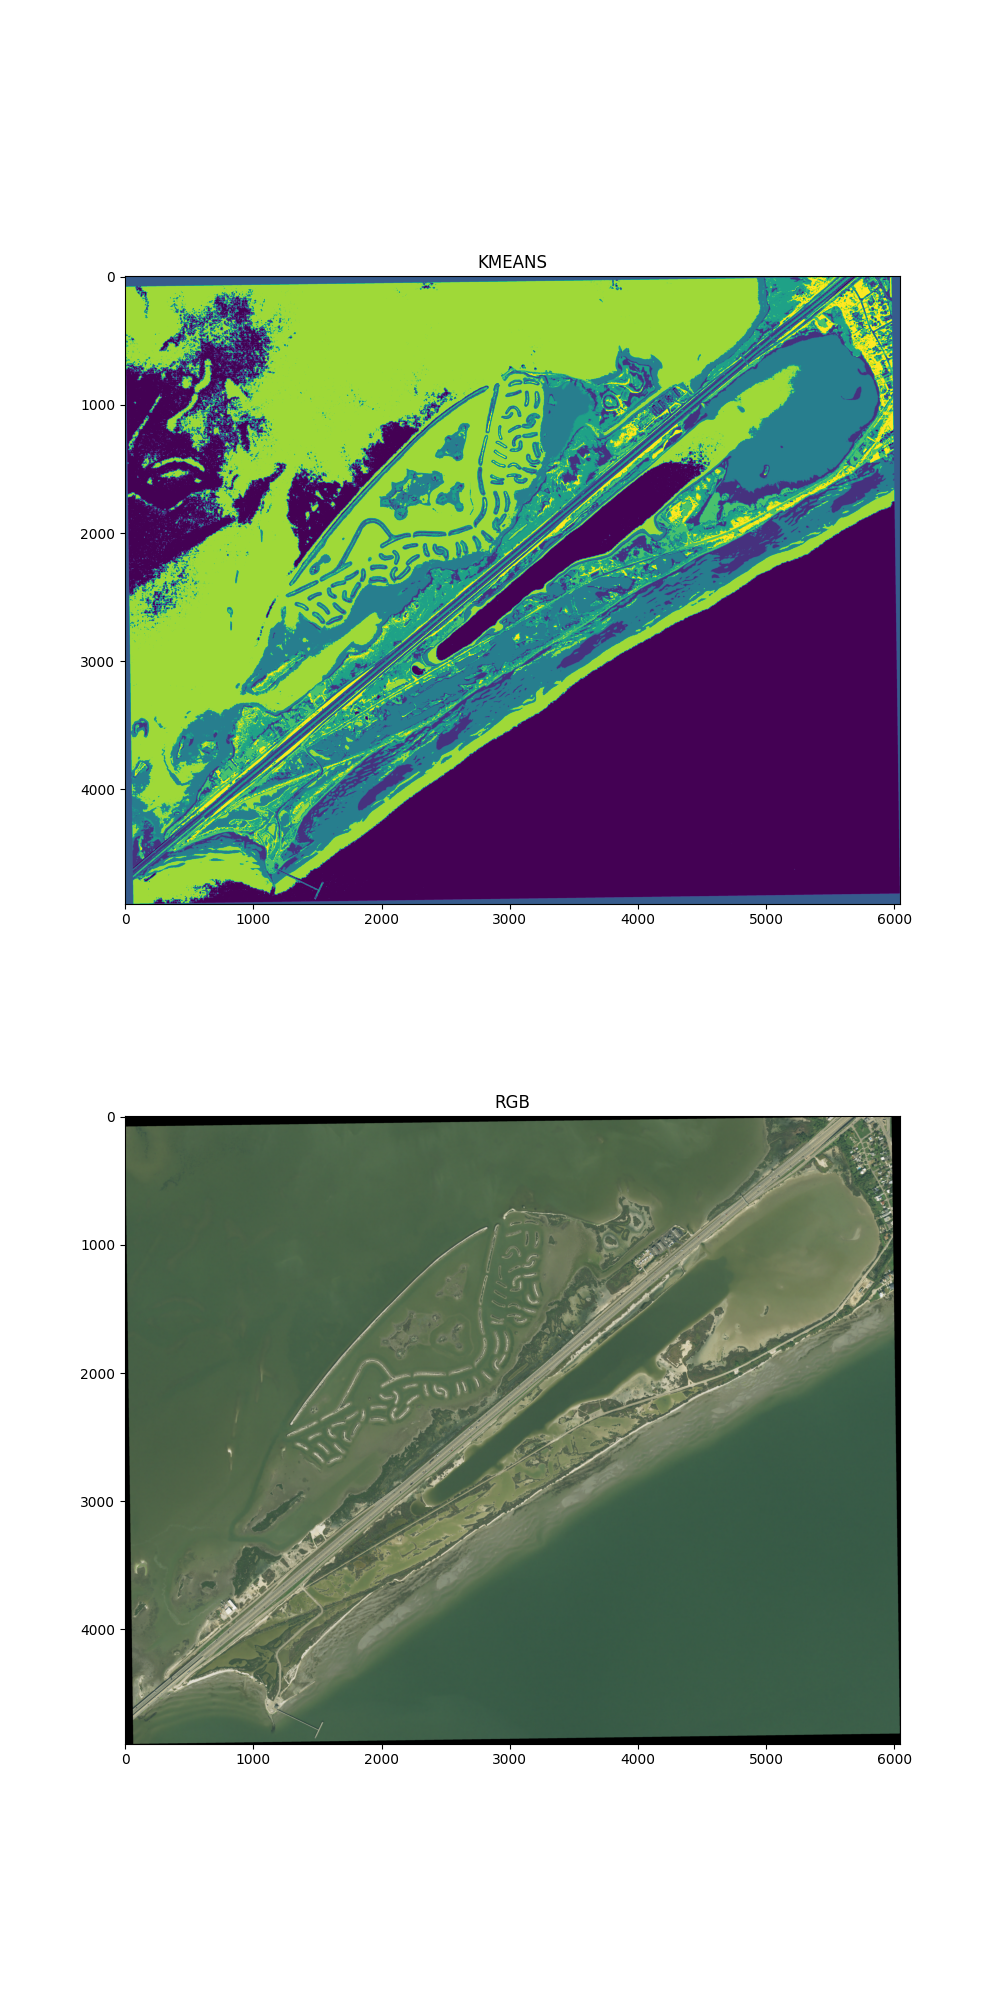
\includegraphics[width=\textwidth,trim={0cm 26cm 0cm 8cm},clip]{img/clusters.png}
            \end{block}
            \begin{itemize}
                \item Via internet/sensors
                \item Assign targets \& reward probabilities
                \item Onboard update via newly acquired data
            \end{itemize}
        \end{column}
        \begin{column}{0.33\textwidth}
            \begin{block}{Mission planning}
            \vspace{.25cm}
                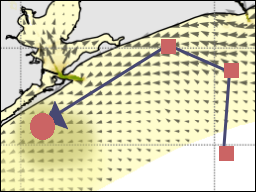
\includegraphics[width=0.75\textwidth,trim={0cm 0cm 0cm 0cm},clip]{img/mission_planning.png}
            \end{block}
            \begin{itemize}
                \item Paths to visit targets
                \item Efficiency based on online weather predictions
                \item Onboard re-routing with new information
            \end{itemize}
        \end{column}
        \begin{column}{0.33\textwidth}
            \begin{block}{Reactive}
            \vspace{.25cm}
                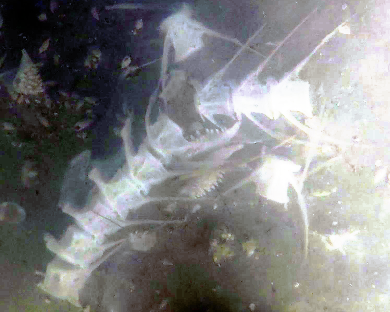
\includegraphics[width=0.9\textwidth,trim={0cm 0cm 0cm 2cm},clip]{img/bones.png}
            \end{block}
            \begin{itemize}
                \item Detect \& pursue outliers, recognized targets
                \item Collision avoidance (above and below waterline)
            \end{itemize}
        \end{column}
    \end{columns}        
    \vspace{1cm}
    
    Here, focused on \textbf{data-driven} \& \textbf{mission planning} aspects.
\end{frame}

\begin{frame}{System Overview}
    \centering
    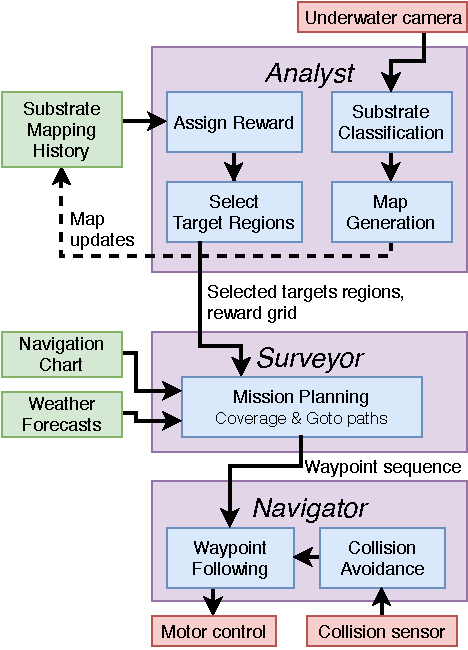
\includegraphics[scale=0.75]{img/system.pdf}
\end{frame}

\begin{frame}{Data-driven reward \& target assignment}
    \begin{enumerate}
        \item Assume map of \textit{entities} available
        \begin{itemize}
            \item What? Could be substrate clusters, uncertainty levels, etc
            \item How? Satellites, aerial imagery, data from \textbf{past USV missions}.
        \end{itemize}
        \item Onboard $\rightarrow$ retarget with new data in seconds
        \item Reward based on static and historical info \\
        Characteristics that could increase reward: \\
        \begin{itemize}
            \item Density $\rightarrow$ favour rarity
            \item Evolution $\rightarrow$ speed \& acceleration
            \item Collection history $\rightarrow$ focus on less-covered entities
        \end{itemize}
    \end{enumerate}
    \vfill
    \begin{block}{Example: algae bloom}
        \begin{columns}
            \begin{column}{0.6\textwidth}
                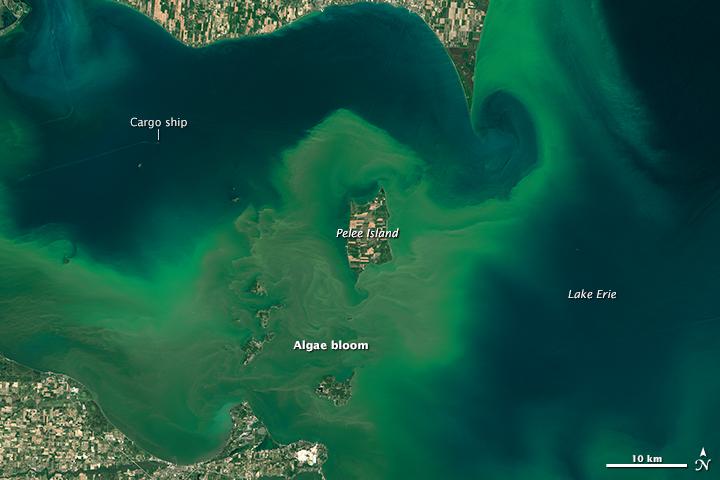
\includegraphics[width=\textwidth,trim={0cm 2cm 2cm 2cm},clip]{img/algae_bloom.jpg} \\
                {\tiny \url{earthobservatory.nasa.gov/images/86327/algae-boom-in-lake-erie}}
                
            \end{column}
            \begin{column}{0.55\textwidth}
                    \begin{itemize}
                        \item Satellites $\rightarrow$ monitor over time
                        \item USV can monitor local interactions, focusing on highly dynamic regions

                    \end{itemize}
            \end{column}            
        \end{columns}
    \end{block}
\end{frame}

\begin{frame}{Data-driven reward: illustrated example}
    \begin{columns}
        \begin{column}{0.25\textwidth}
            Entities, t + 0
            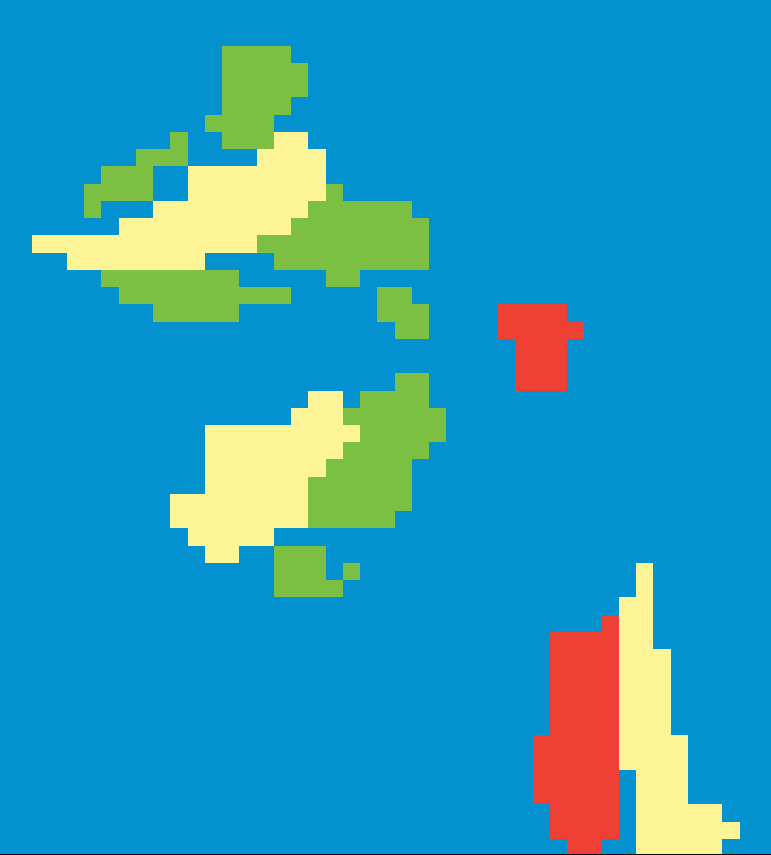
\includegraphics[width=\textwidth,trim={0cm 0cm 0cm 0cm},clip]{img/ep0.png}
        \end{column}
        \begin{column}{0.25\textwidth}
            Entities, t + $\Delta$ t
            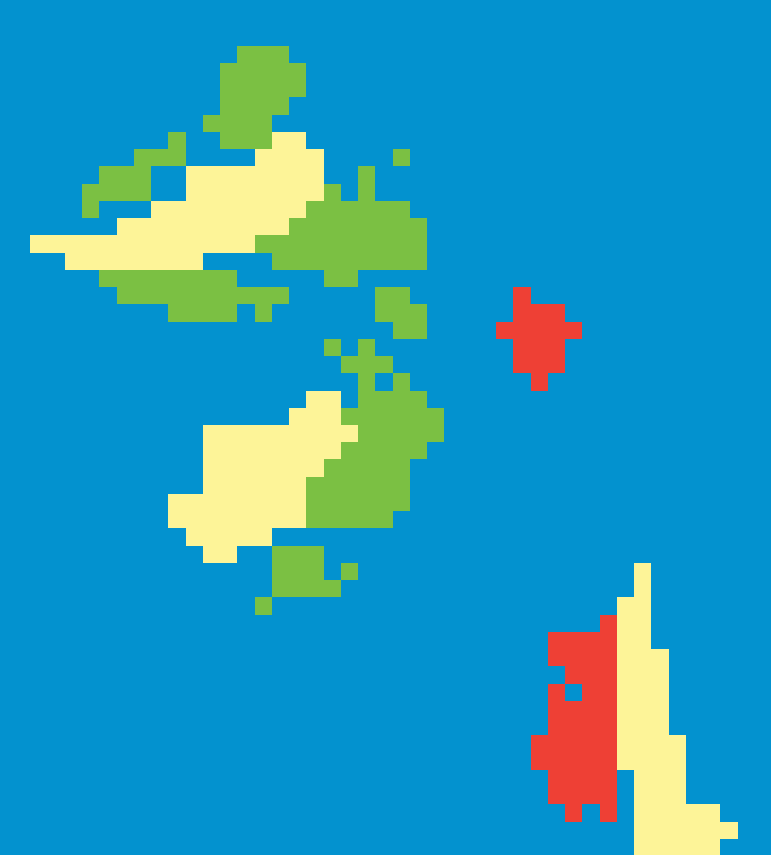
\includegraphics[width=\textwidth,trim={0cm 0cm 0cm 0cm},clip]{img/ep1.png}
        \end{column}
        \begin{column}{0.25\textwidth}
            Entities, t + 2 $\Delta$ t
            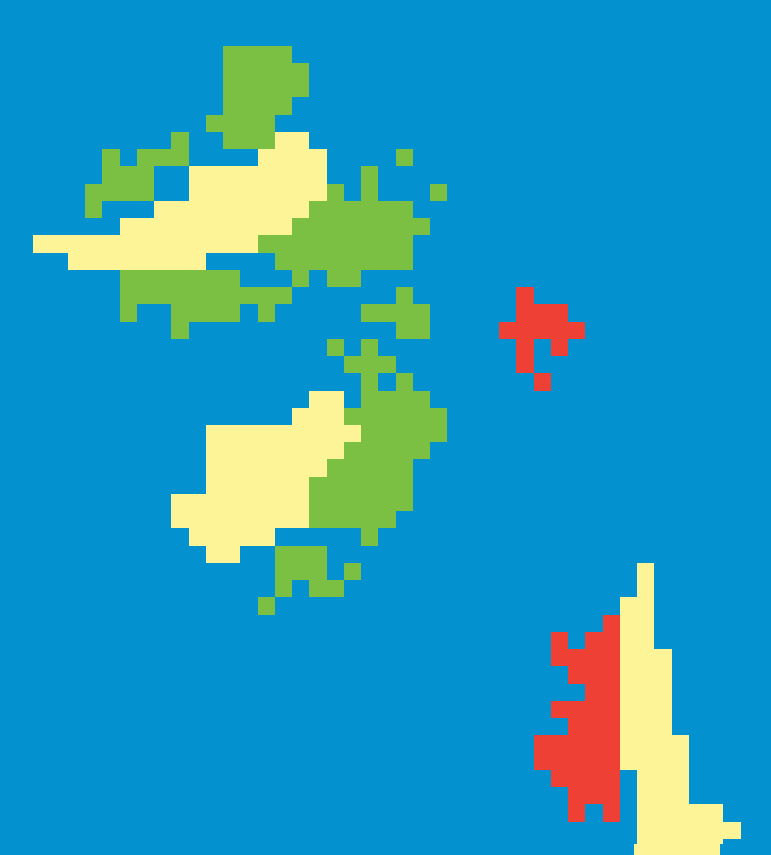
\includegraphics[width=\textwidth,trim={0cm 0cm 0cm 0cm},clip]{img/ep2.png}
        \end{column}
        \begin{column}{0.25\textwidth}
        Reward assignment
            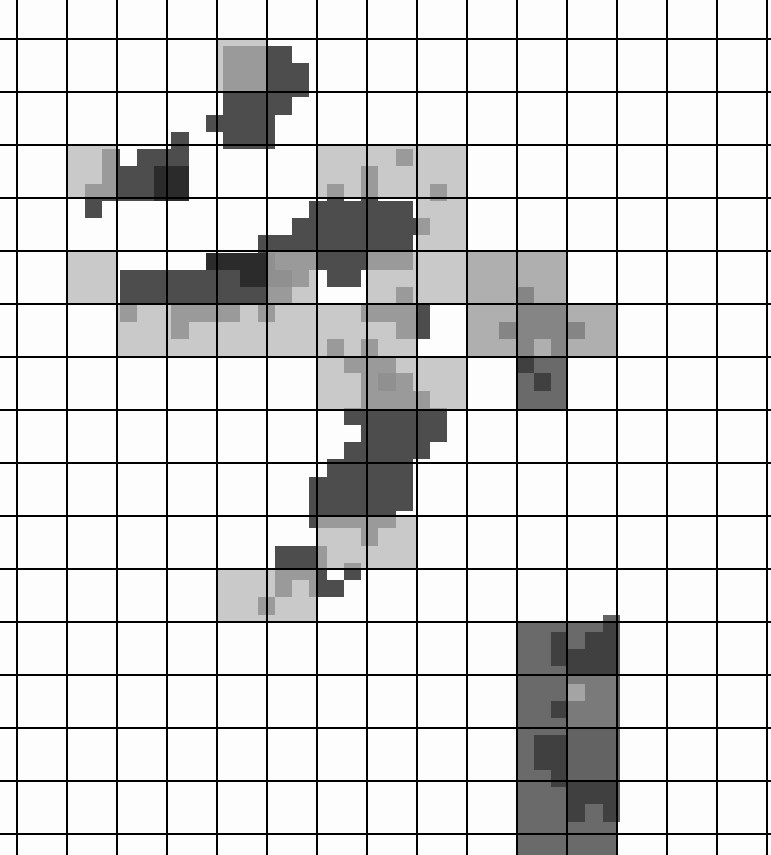
\includegraphics[width=\textwidth,trim={0cm 0cm 0cm 0cm},clip]{img/epreward.png}
        \end{column}
    \end{columns}
    
    \begin{itemize}
        \item A simple, illustrative example assignment scheme:
        \begin{enumerate}
            \item Calculate proportion of each entity
            \item Init reward grid with zeros (same dimensions as maps)
            \item For each cell in reward grid:
            \begin{itemize}
                \item Increase reward if entity present, weighted by entity's rarity
            \end{itemize}
            \item Divide into NxN blocks
            \item For each block:
            \begin{enumerate}
                \item Calculate entity speed, acceleration across history
                \item Increase reward for all pixels in block based on speed and acceleration
            \end{enumerate}
        \end{enumerate}
        \item Motivation 1: onboard reward assignment \\
        Update the current map $\rightarrow$ new reward in $<0.1$ seconds \\ (for 1000 x 1000 maps)
        \item Motivation 2: sensible results with very little data \\ Avoid data-hungry machine learning techniques
    \end{itemize}
\end{frame}
\begin{frame}{Mission planning: minimizing energy \& maximizing reward}
    \begin{enumerate}
        \item Energy efficient
        \begin{itemize}
            \item Access online surface current, wind model outputs
            \item Temporal: have set of discrete future predictions
            \item Minimize work done by vessel to maintain target velocity
        \end{itemize}
        \item Opportunistic reward
        \begin{itemize}
            \item Take advantage of nearby reward on route to target
        \end{itemize}
        \item Fast for onboard planning
        \begin{itemize}
            \item Need path within seconds
            \item Willing to sacrifice optimality
            \item Improve path while vehicle underway
        \end{itemize}
    \end{enumerate}
    
    \begin{columns}
        \begin{column}{0.5\textwidth}
    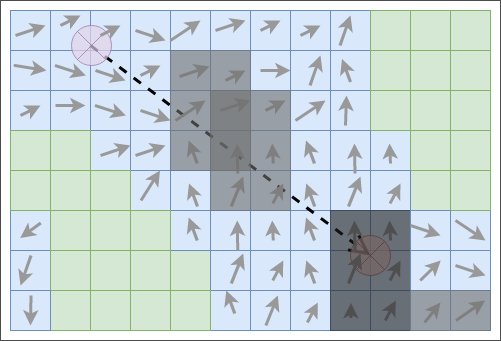
\includegraphics[width=\textwidth,trim={0cm 0cm 0cm 0cm},clip]{img/segment_.png} \\
        {\tiny Path segment. Darker blue $\rightarrow$ higher reward.}
        \end{column}
        \begin{column}{0.5\textwidth}
            \begin{block}{Metaheuristic fitness function}
                \begin{itemize}
                    \item Evaluates a sequence of waypoints
                    \item All cells along path used to calculate work, reward, and obstacle penalty
                    \item After each cell, updates estimated duration to interpolate water currents value
                \end{itemize}
            \end{block}
        \end{column}        
    \end{columns}
    
\end{frame}

\begin{frame}{Environment for Simulation Experiments}
    \begin{columns}
        \begin{column}{0.5\textwidth}
        \centering
            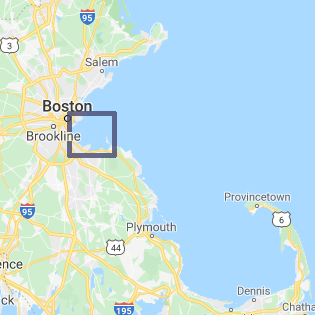
\includegraphics[width=0.65\textwidth,trim={0cm 0cm 0cm 0cm},clip]{img/large.png}
        \end{column}    
        \begin{column}{0.5\textwidth}
            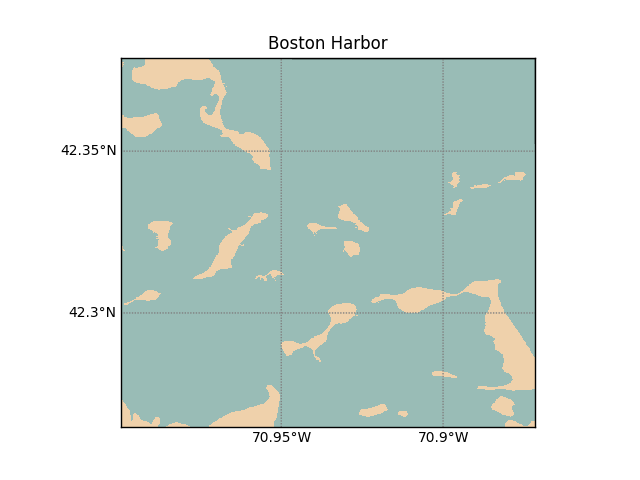
\includegraphics[width=\textwidth,trim={0cm 0cm 0cm 0cm},clip]{img/full.png}
        \end{column}
    \end{columns}
    \begin{columns}
        \begin{column}{0.5\textwidth}
            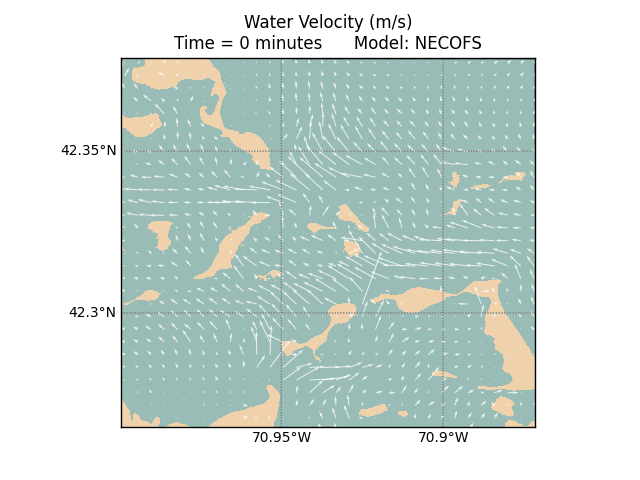
\includegraphics[width=\textwidth,trim={0cm 0cm 0cm 0cm},clip]{img/full_water_1.png}
        \end{column}
        \begin{column}{0.5\textwidth}
            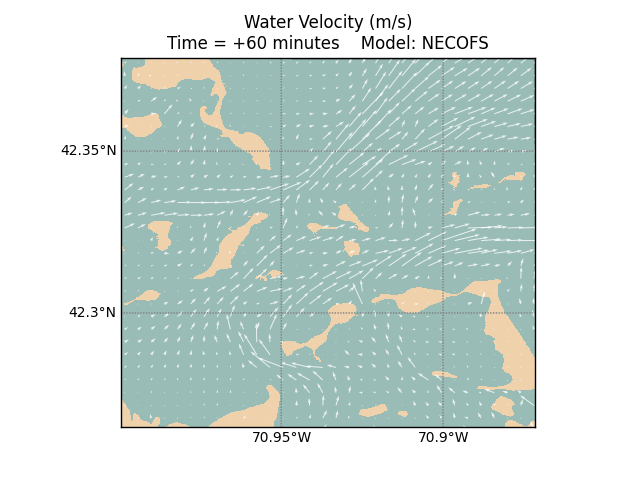
\includegraphics[width=\textwidth,trim={0cm 0cm 0cm 0cm},clip]{img/full_water_2.png}
        \end{column}
    \end{columns}
\end{frame}

\begin{frame}{Environment}
    \begin{columns}
        \begin{column}{0.5\textwidth}
            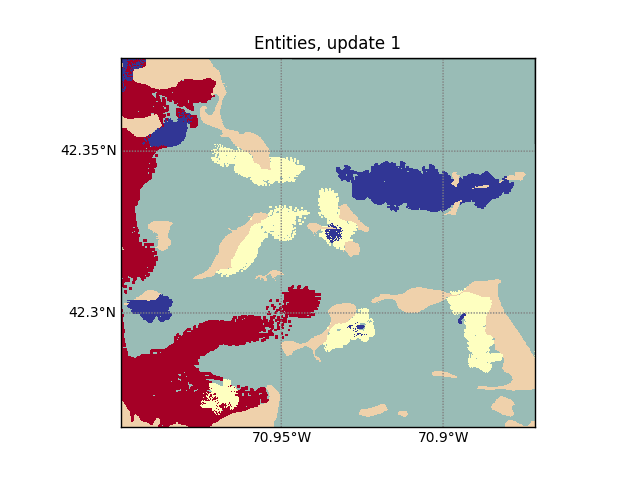
\includegraphics[width=\textwidth,trim={0cm 0cm 0cm 0cm},clip]{img/e1.png}
        \end{column}
        \begin{column}{0.5\textwidth}
            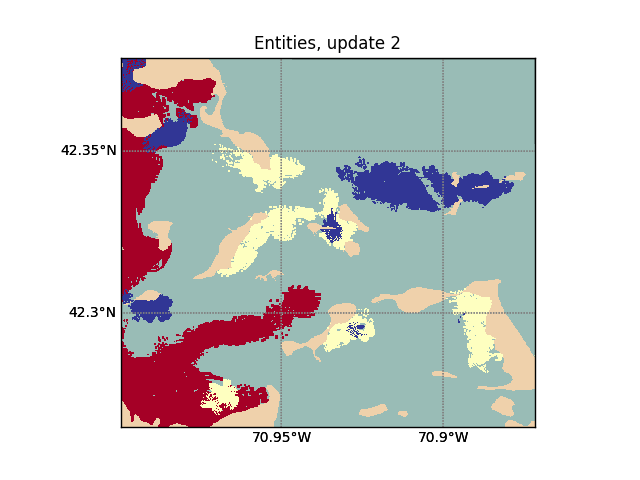
\includegraphics[width=\textwidth,trim={0cm 0cm 0cm 0cm},clip]{img/e2.png}
        \end{column}
    \end{columns}
    \begin{columns}
        \begin{column}{0.5\textwidth}
            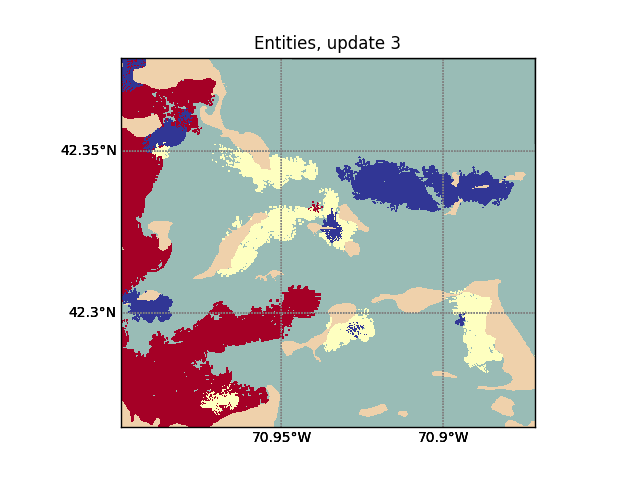
\includegraphics[width=\textwidth,trim={0cm 0cm 0cm 0cm},clip]{img/e3.png}
        \end{column}
        \begin{column}{0.5\textwidth}
            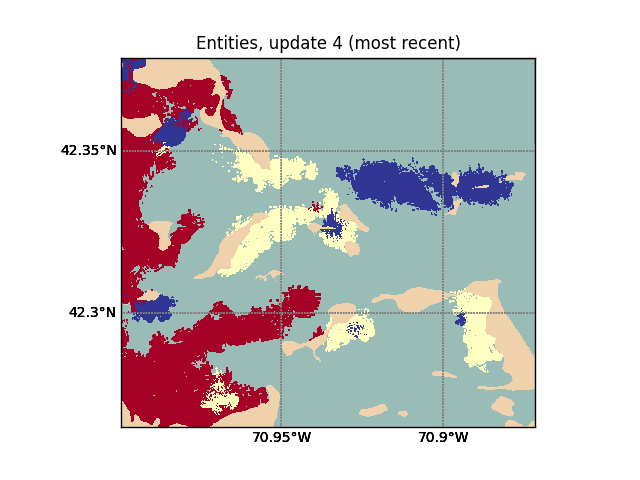
\includegraphics[width=\textwidth,trim={0cm 0cm 0cm 0cm},clip]{img/e4.png}
        \end{column}
    \end{columns}
\end{frame}

\begin{frame}{Comparing efficiency of PSO to A* for energy-minimizing planning}
    \begin{columns}
        \begin{column}{0.5\textwidth}
            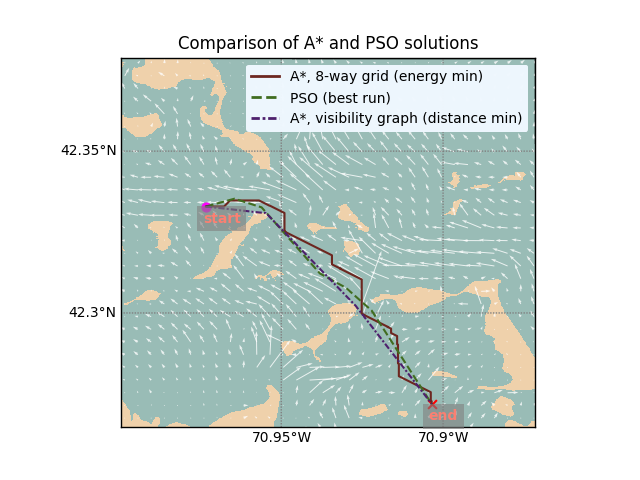
\includegraphics[width=\textwidth,trim={0cm 0cm 0cm 0cm},clip]{img/paths_FP2_compare.png}
        \end{column}
        \begin{column}{0.5\textwidth}
            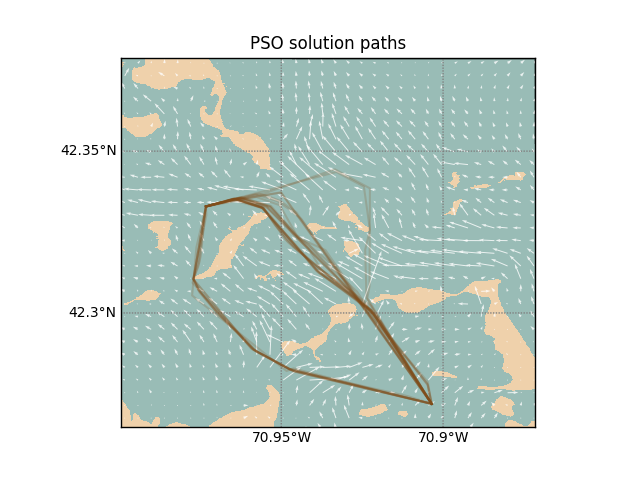
\includegraphics[width=\textwidth,trim={0cm 0cm 0cm 0cm},clip]{img/paths_FP2_many.png}
        \end{column}        
    \end{columns}
    \begin{columns}
        \begin{column}{0.5\textwidth}
            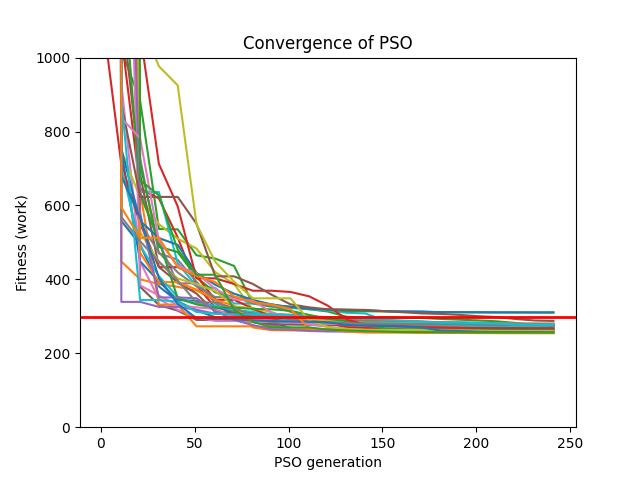
\includegraphics[width=\textwidth,trim={0cm 0cm 0cm 0cm},clip]{img/FP2_convergence.png}
        \end{column}
        \begin{column}{0.5\textwidth}
            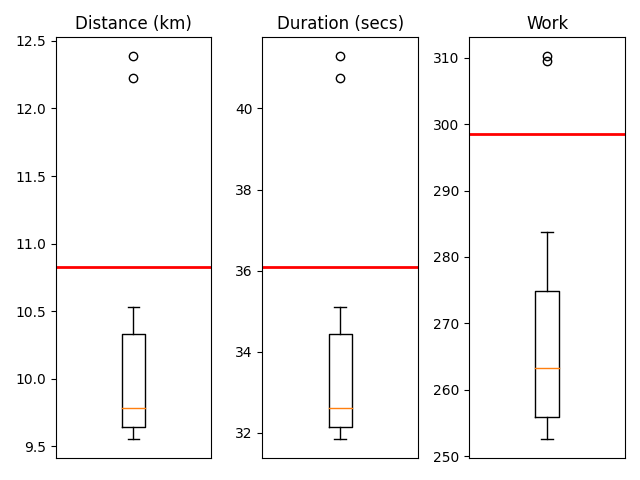
\includegraphics[width=\textwidth,trim={0cm 0cm 0cm 0cm},clip]{img/FP2_box.png}
        \end{column}
    \end{columns}
\end{frame}

\begin{frame}{Comparing efficiency of PSO to A* for energy-minimizing planning}
    \begin{columns}
        \begin{column}{0.5\textwidth}
            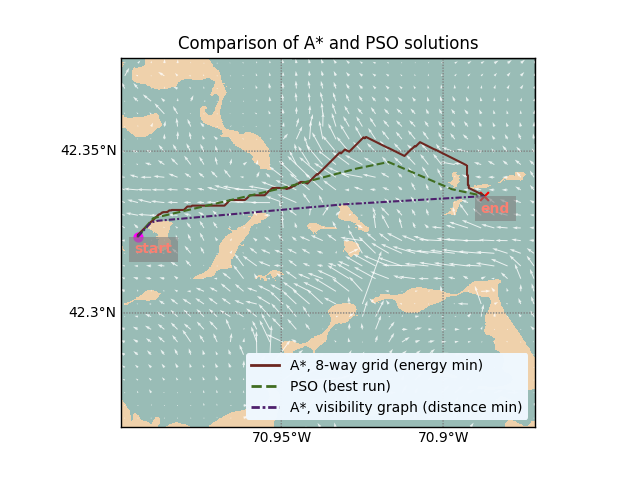
\includegraphics[width=\textwidth,trim={0cm 0cm 0cm 0cm},clip]{img/paths_FP1_compare.png}
        \end{column}
        \begin{column}{0.5\textwidth}
            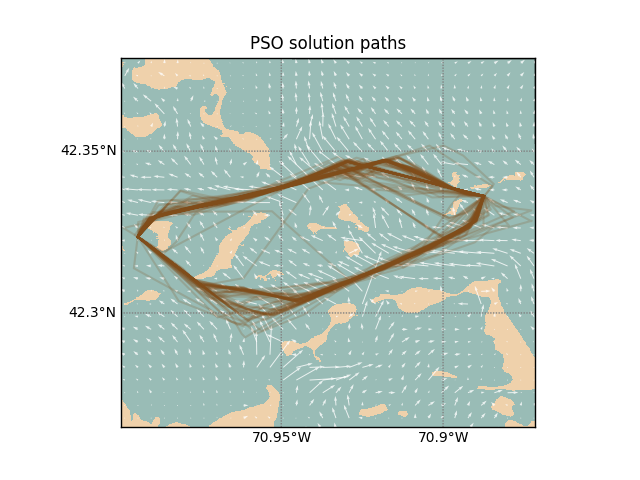
\includegraphics[width=\textwidth,trim={0cm 0cm 0cm 0cm},clip]{img/paths_FP1_many.png}
        \end{column}        
    \end{columns}
    \begin{columns}
        \begin{column}{0.5\textwidth}
            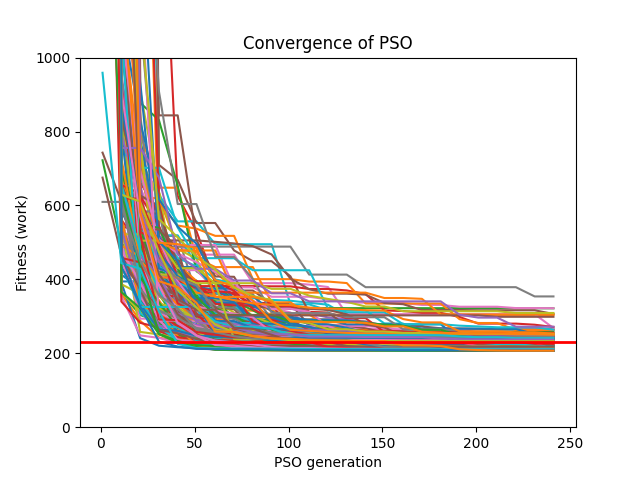
\includegraphics[width=\textwidth,trim={0cm 0cm 0cm 0cm},clip]{img/FP1_convergence.png}
        \end{column}
        \begin{column}{0.5\textwidth}
            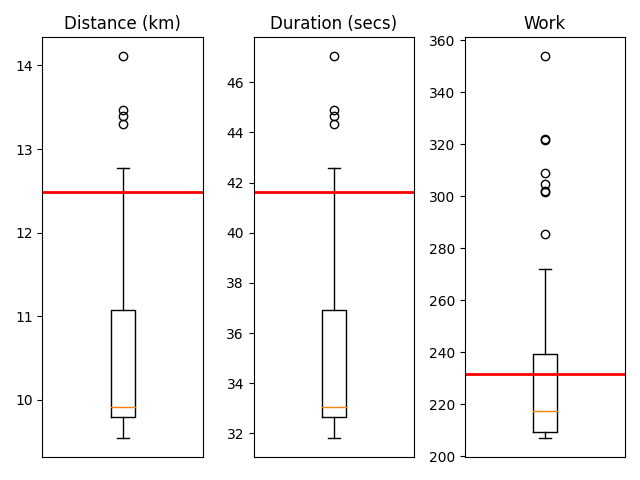
\includegraphics[width=\textwidth,trim={0cm 0cm 0cm 0cm},clip]{img/FP1_box.png}
        \end{column}
    \end{columns}
\end{frame}

\begin{frame}{Incorporating reward maximization}
    \begin{columns}
        \begin{column}{0.33\textwidth}
            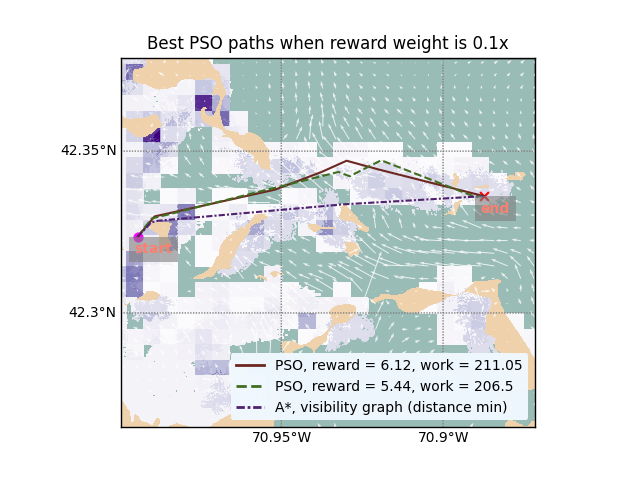
\includegraphics[width=1.2\textwidth,trim={3cm 0cm 0cm 0cm},clip]{img/paths_FP1_RW0.1.png}
        \end{column}
        \begin{column}{0.31\textwidth}
            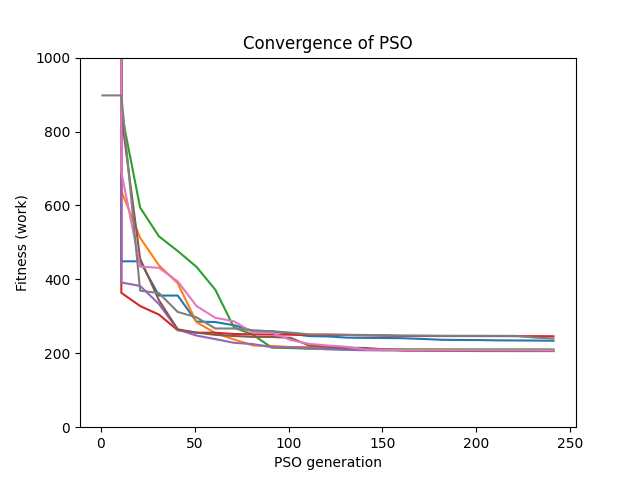
\includegraphics[width=\textwidth,trim={0cm 0cm 2.5cm 0cm},clip]{img/FP1_RW0.1_convergence.png}
        \end{column}
        \begin{column}{0.37\textwidth}
            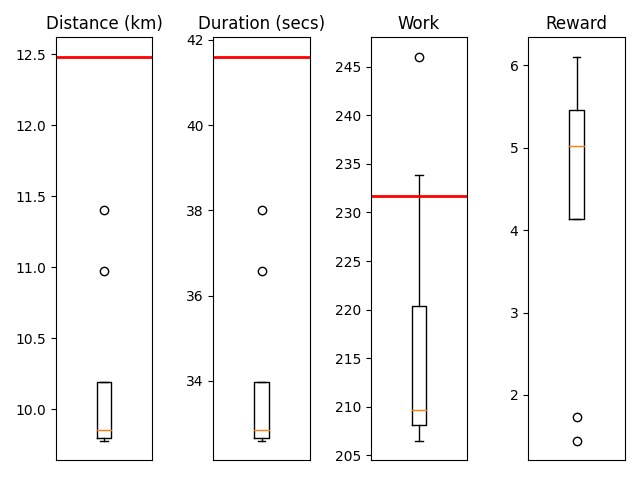
\includegraphics[width=\textwidth,trim={0cm 0cm 0cm 0cm},clip]{img/FP1_RW0.1__box.png}
        \end{column}
    \end{columns}
    \begin{columns}
        \begin{column}{0.33\textwidth}
            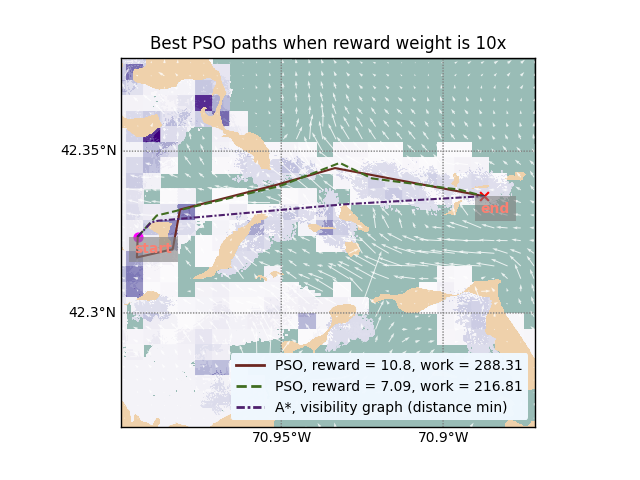
\includegraphics[width=1.2\textwidth,trim={3cm 0cm 0cm 0cm},clip]{img/paths_FP1_RW10.png}
        \end{column}
        \begin{column}{0.31\textwidth}
            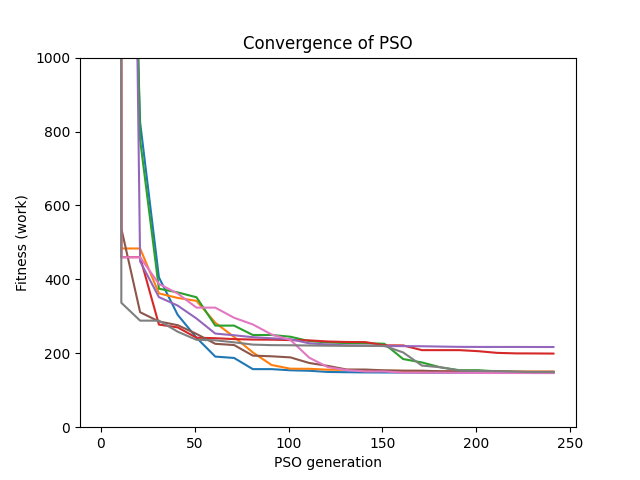
\includegraphics[width=\textwidth,trim={0cm 0cm 2.5cm 0cm},clip]{img/FP1_RW10_convergence.png}
        \end{column}
        \begin{column}{0.37\textwidth}
            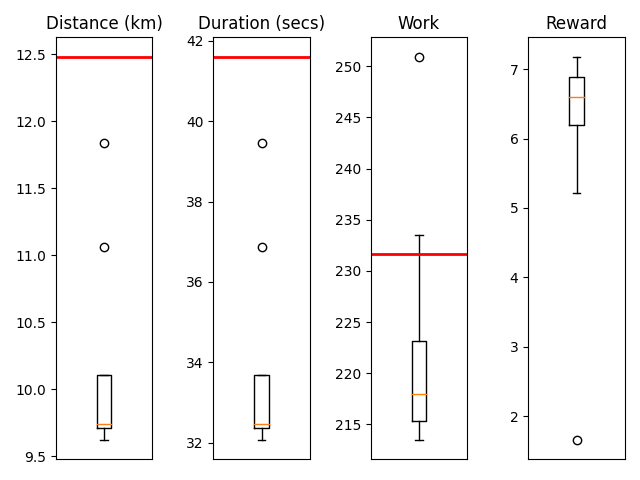
\includegraphics[width=\textwidth,trim={0cm 0cm 0cm 0cm},clip]{img/FP1_RW10_box.png}
        \end{column}
    \end{columns} 
\end{frame}
\begin{frame}{Collecting data to update maps}
    \begin{itemize}
        \item So far, have assumed map of \textit{entities} available
        \item In turbid waters, limited information from aerial imagery \\
        Some of the below clusters are seagrass meadows, others just depth levels
    \end{itemize}
    \begin{columns}
        \begin{column}{0.5\textwidth}
        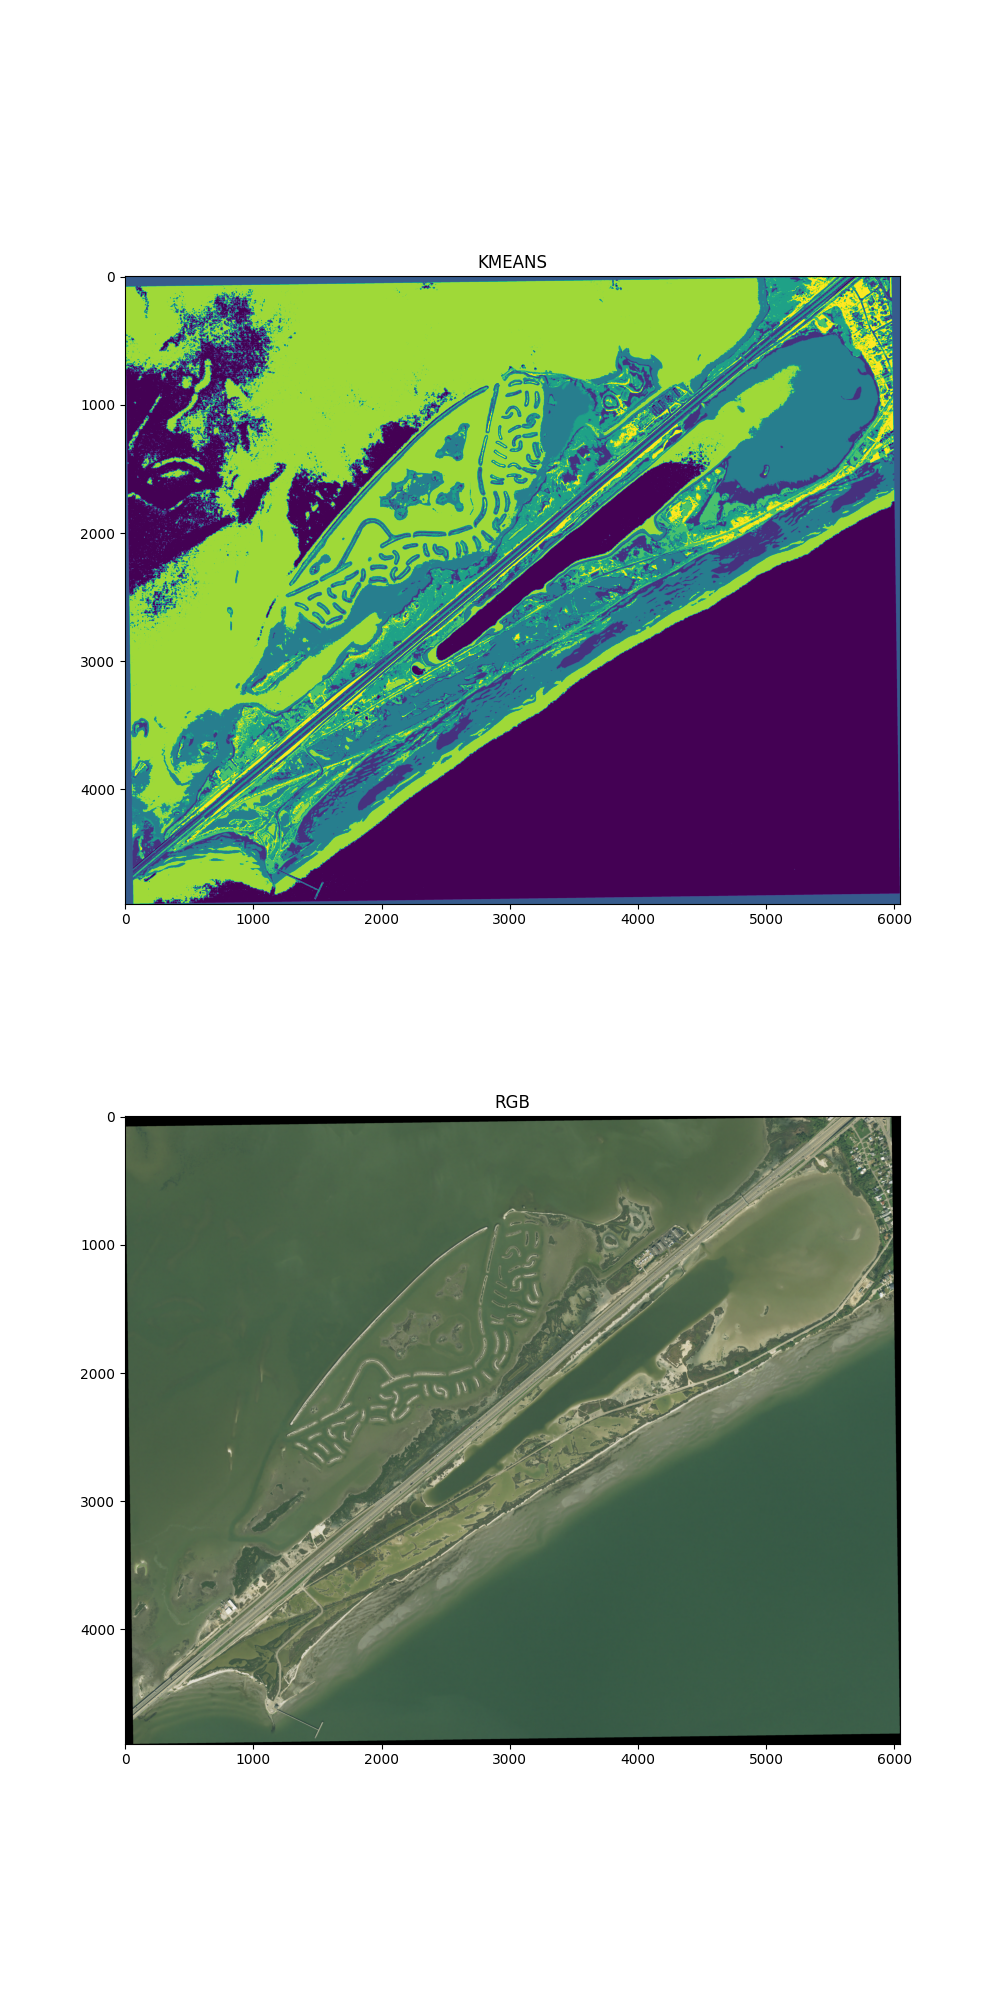
\includegraphics[width=0.8\textwidth,trim={4cm 9cm 4cm 33cm},clip]{img/clusters.png}  
        \end{column}    
        \begin{column}{0.5\textwidth}
        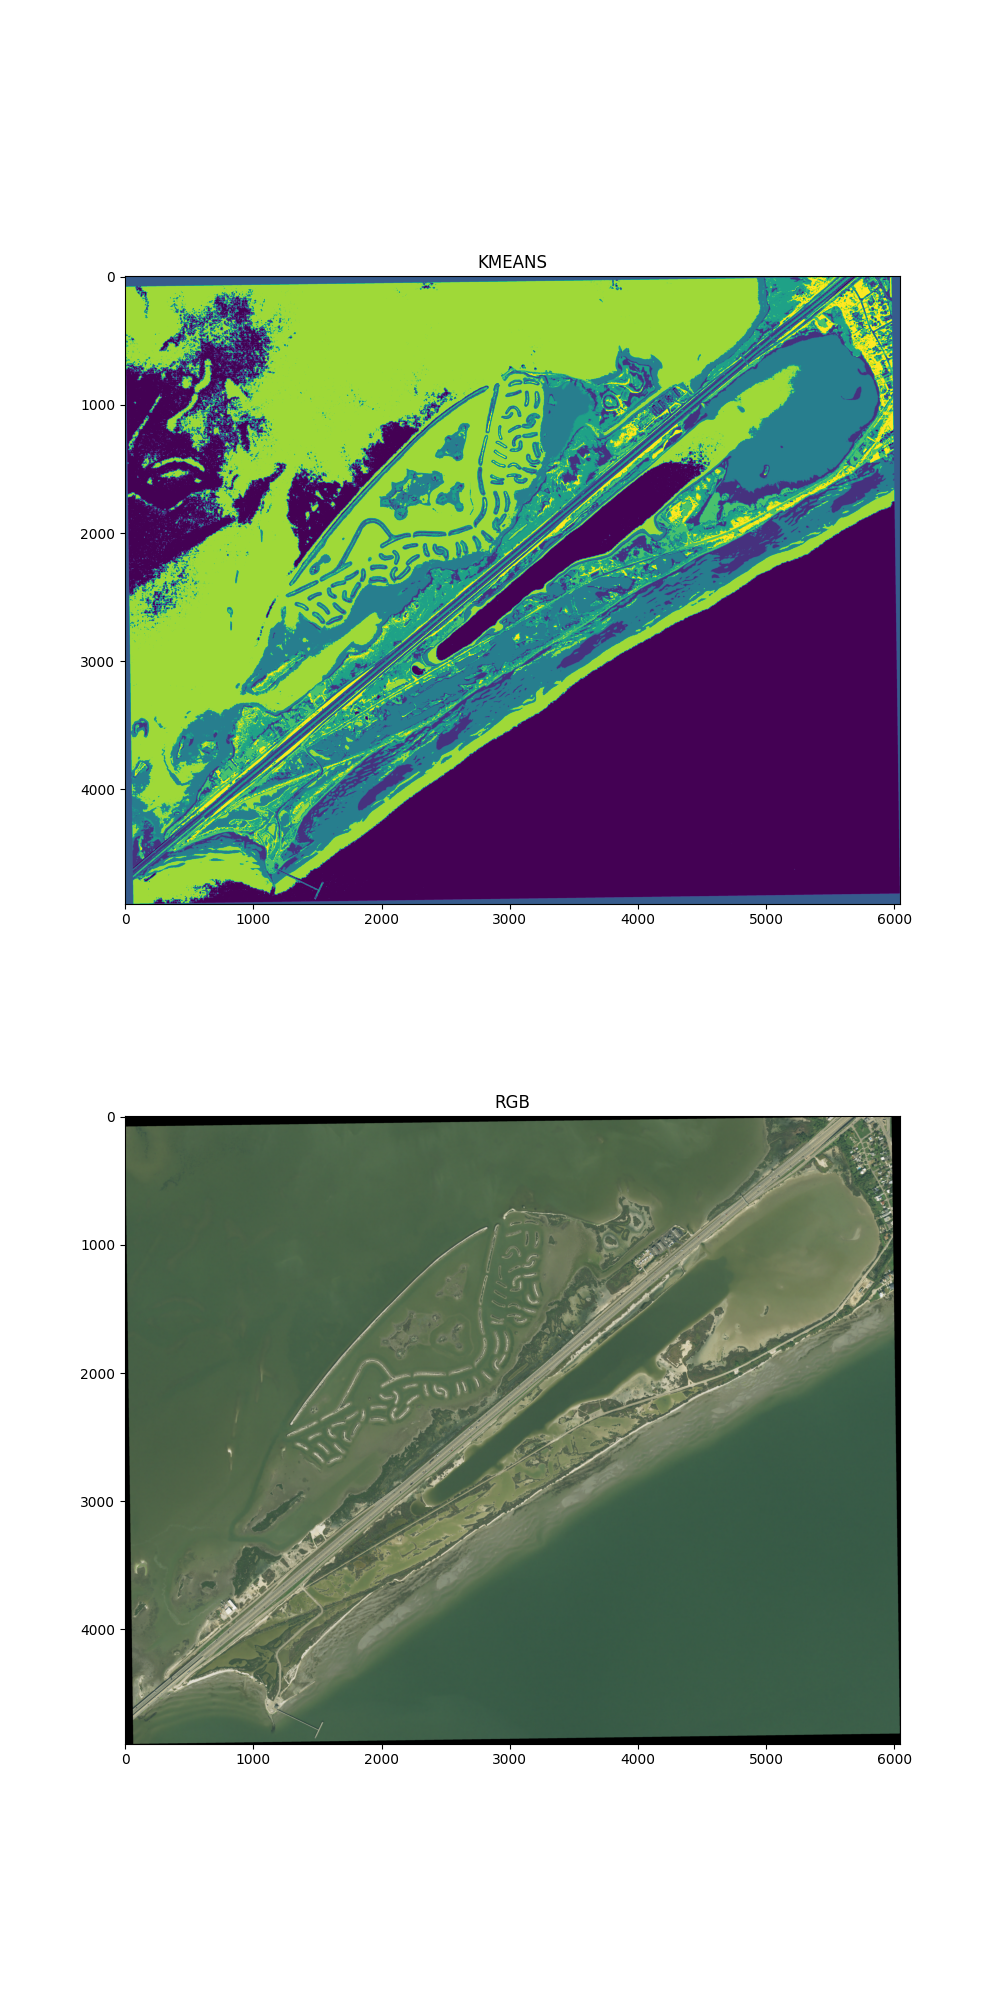
\includegraphics[width=0.8\textwidth,trim={4cm 30cm 4cm 12cm},clip]{img/clusters.png}
        \end{column}
    \end{columns}
    \begin{itemize}
        \item But this is why we have an explorer USV
        \item Idea: use initial map from aerial image, \\
        explore to reduce uncertainty, discriminate clusters, and find more entities
    \end{itemize}
    \begin{block}{GoPro Hero 4 underwater imagery}
        \begin{itemize}
            \item Collected in the Laguna Madre, Corpus Christ, Texas
            \item Characterized by very high turbidity
        \end{itemize}
        \begin{columns}
            \begin{column}{0.33\textwidth}
            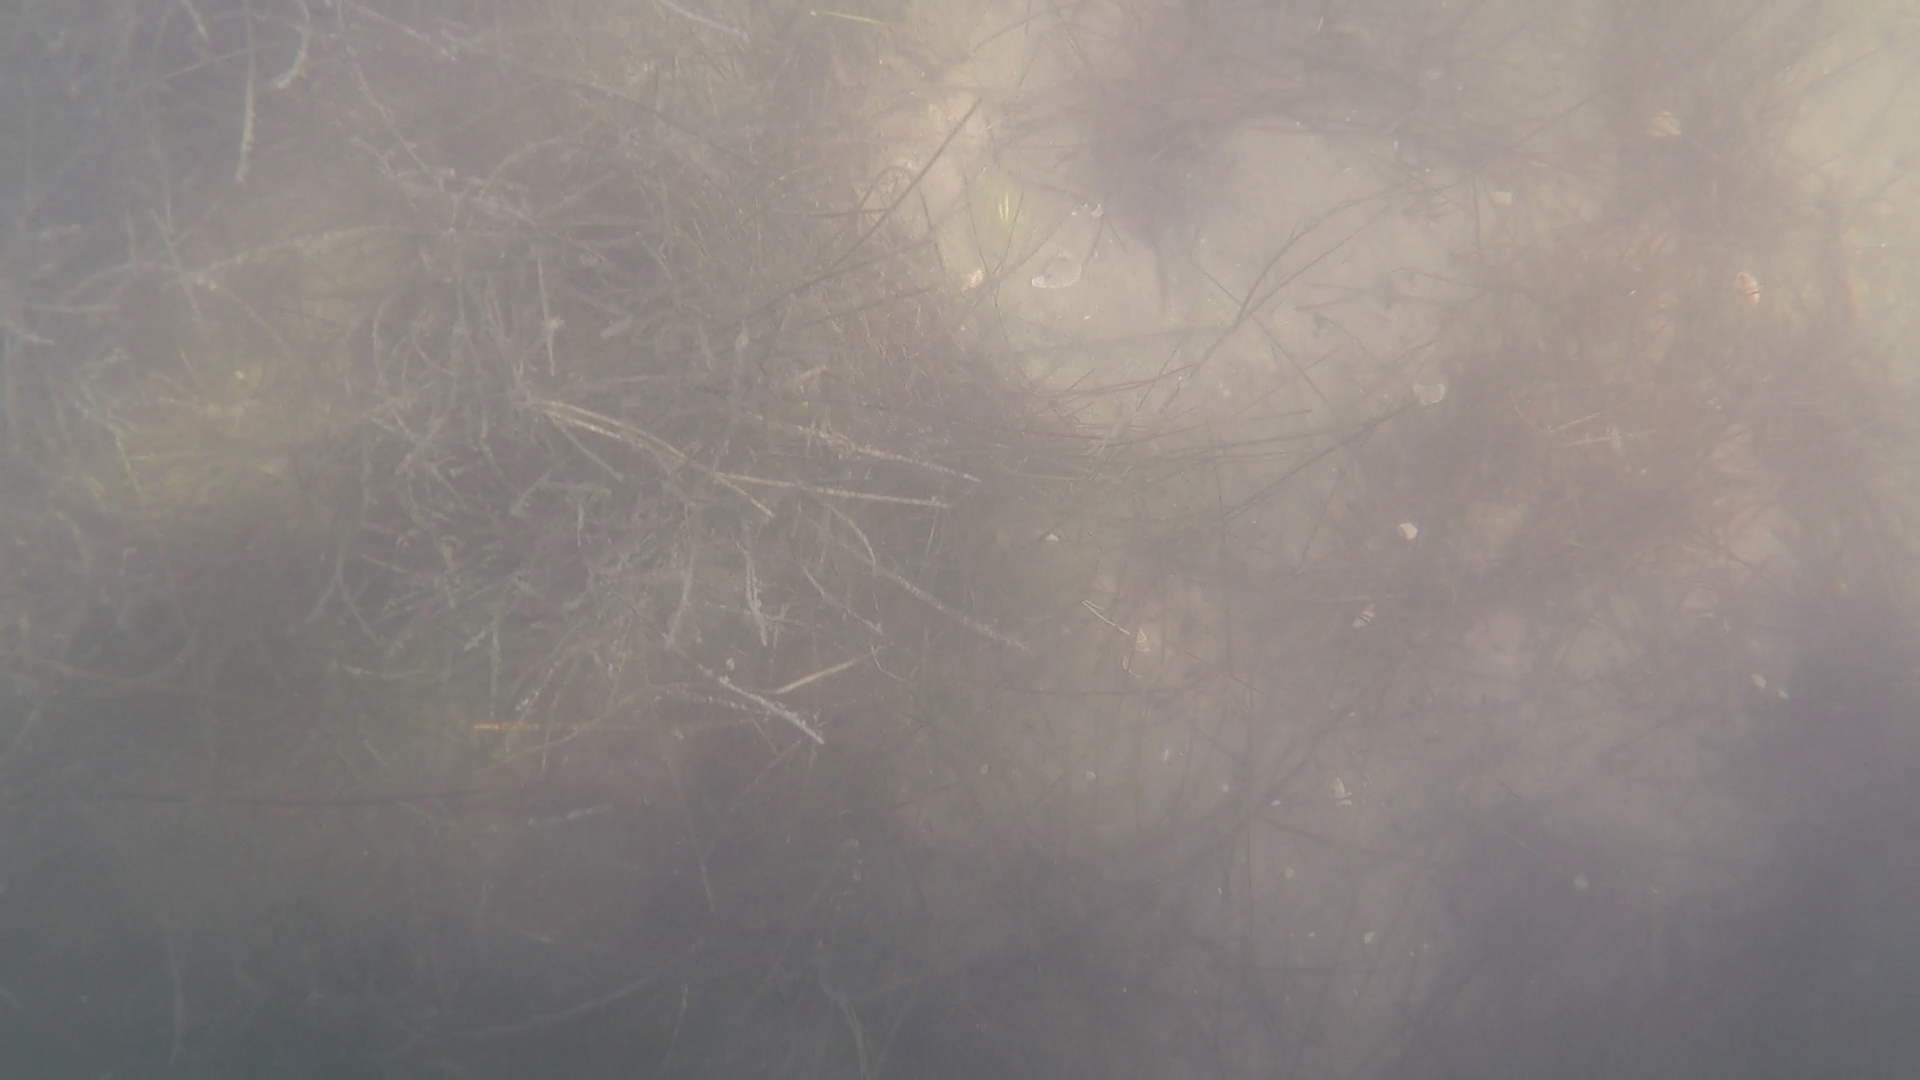
\includegraphics[width=\textwidth,trim={0cm 0cm 0cm 0cm},clip]{img/seagrass_field1_file2-00002.png}
            \end{column}
            \begin{column}{0.33\textwidth}
            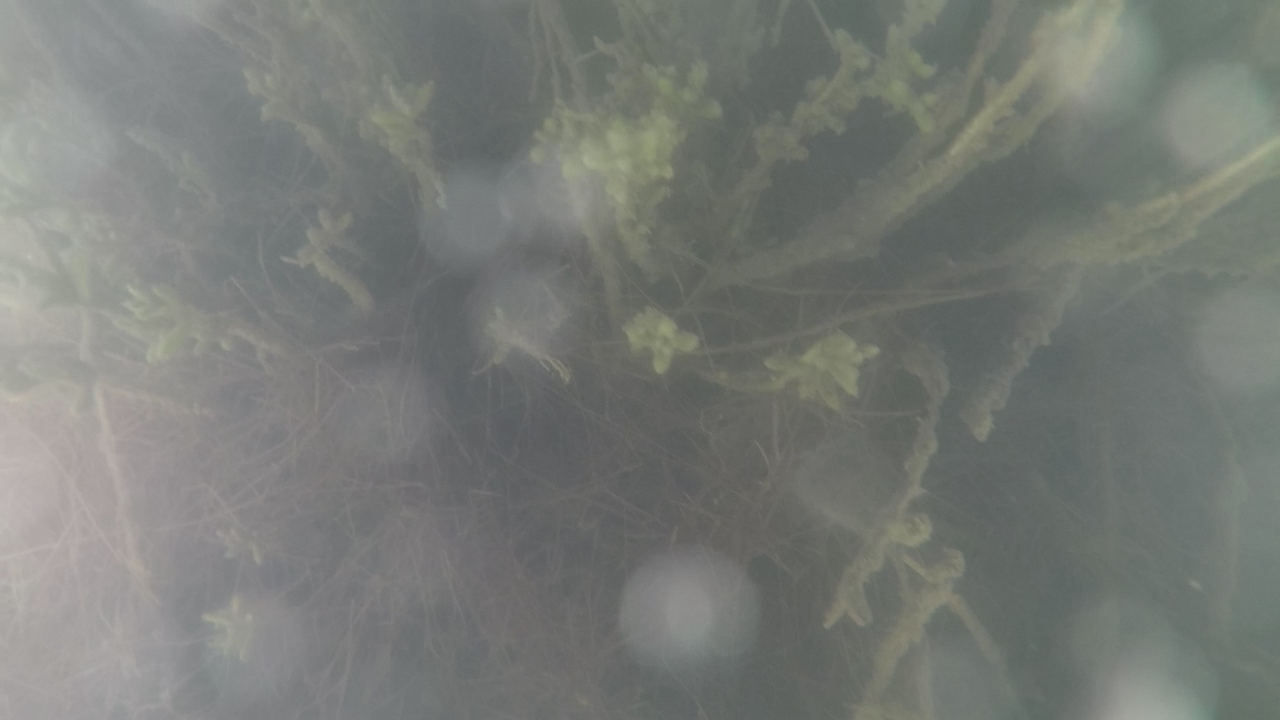
\includegraphics[width=\textwidth,trim={0cm 0cm 0cm 0cm},clip]{img/seagrass_field2_file1-00039.png}
            \end{column}
            \begin{column}{0.33\textwidth}
            
\includegraphics[width=\textwidth,trim={0cm 0cm 0cm 0cm},clip]{img/seagrass_field2_file2-00057.png}      \end{column}
        \end{columns}
    \end{block}
\end{frame}
\begin{frame}{Collection data to update maps}
    \begin{block}{Onboard mapping prototype}
        \begin{enumerate}
            \item Image enhancement \\
        \begin{columns}
            \begin{column}{0.33\textwidth}
            {\tiny Original}
            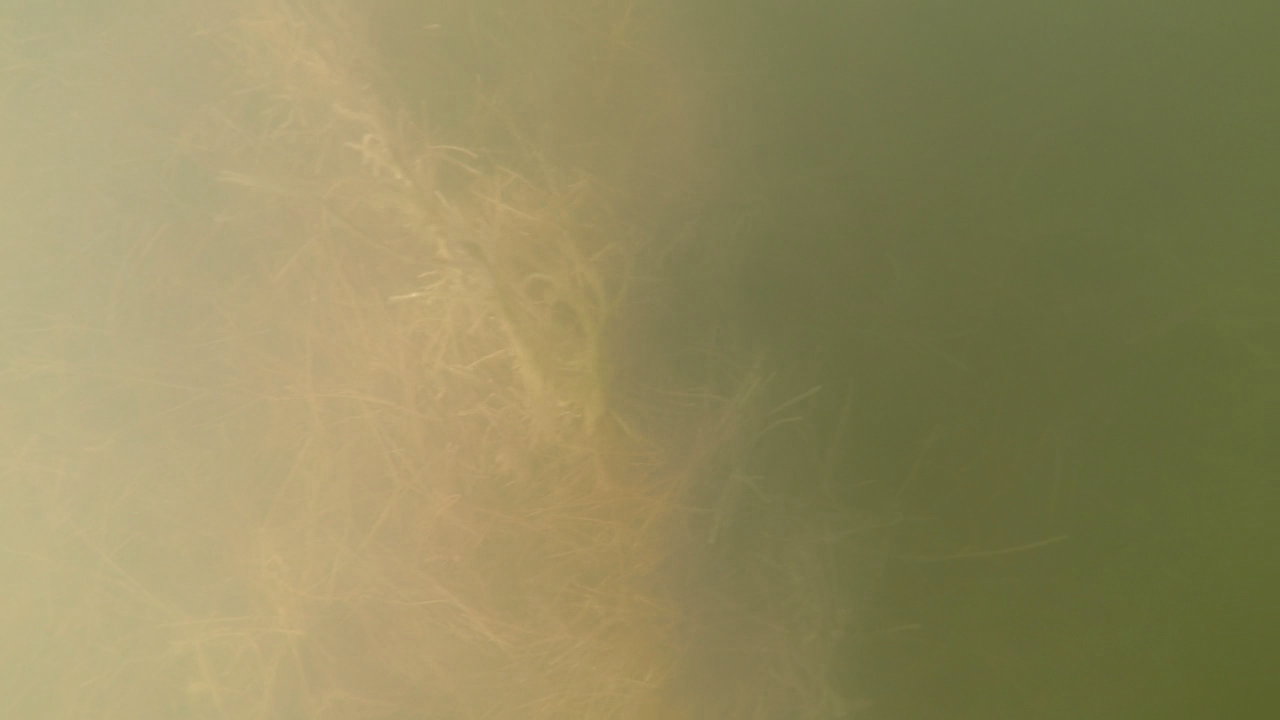
\includegraphics[width=\textwidth,trim={0cm 0cm 0cm 0cm},clip]{img/orig.png}
            \end{column}
            \begin{column}{0.33\textwidth}
            {\tiny White balance via gray-world assumption}
            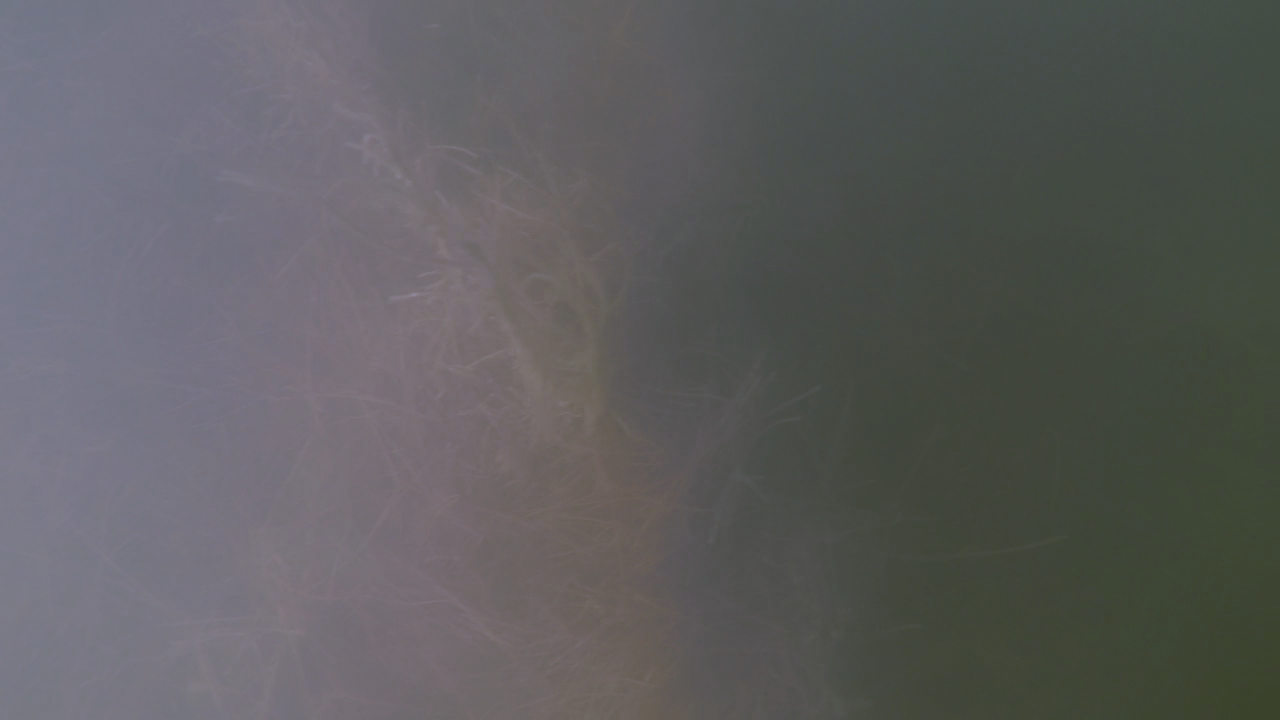
\includegraphics[width=\textwidth,trim={0cm 0cm 0cm 0cm},clip]{img/whiteBalance.png}
            \end{column}
            \begin{column}{0.33\textwidth}
            {\tiny Contrast Limited Adaptive Histogram Eq.}
            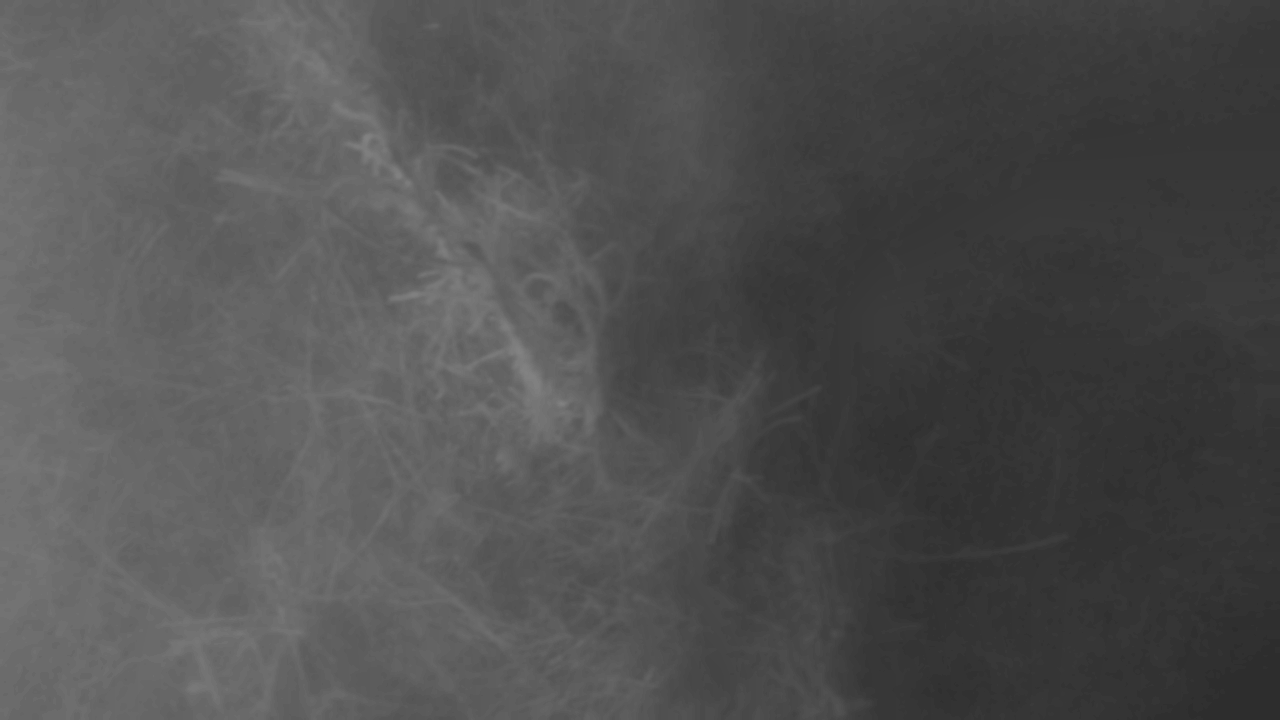
\includegraphics[width=\textwidth,trim={0cm 0cm 0cm 0cm},clip]{img/clahe.png}  
            \end{column}
        \end{columns}
            \item Feature extraction: canny, sobel, laplacian kernels
            \item Decision tree classification  \\
            Mean cross-stratified validation: 82.31\%
            \item Initial onboard mapping result \\
        \begin{columns}
            \begin{column}{0.3\textwidth}
            \centering
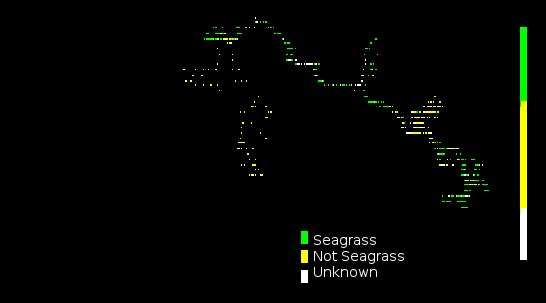
\includegraphics[width=0.9\textwidth,trim={6cm 0cm 1cm 0cm},clip]{img/seagrass_map.png}
            \end{column}
            \begin{column}{0.7\textwidth}
                \begin{itemize}
                    \item High image overlap in shallows $\rightarrow$ \\ use most assigned class
                    \item In-field estimated accuracy $>90\%$
                    \item Onboard mapping: image to decision in $<0.5$ secs
                \end{itemize}
            \end{column}
        \end{columns}  
        \end{enumerate}
    \end{block}
\end{frame}
\begin{frame}{Conclusions}
    \begin{enumerate}
        \item Analyst: target \& reward assignment
        \begin{itemize}
            \item Data-generic technique proposed
            \item Fast online updates when new data available
        \end{itemize}
        \item Surveyor: path planning that balances efficiency and reward
        \begin{itemize}
            \item Limited deviation from efficiency to take advantage of reward opportunities
            \item Exploit PSO's premature convergence for online planning
            \item As PSO converges, the solution improves (while boat underway)
        \end{itemize}
        \item Analyst: onboard image enhancement \& classficication for mapping
        \begin{itemize}
            \item Mapping \textit{entities} allows the explorer to build the history that can be used for target \& reward assignment
        \end{itemize}
    \end{enumerate}
\end{frame}

\end{document}
